\subsection{T90}
\begin{figure}[ht]
\centering
 \captionsetup{width=.68\textwidth}
{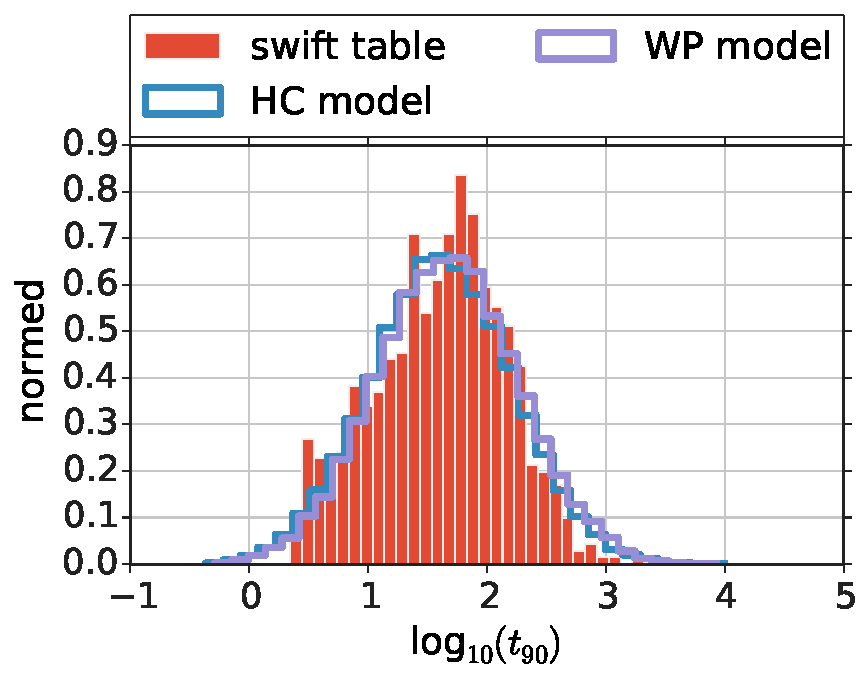
\includegraphics[width=0.68\textwidth]{fig/t90earth.pdf}}
    \caption{The $t_{90}$ distributions at earth based on data extracted from
the Swift database (reference ???) and the drawn distributions based on
$t_{90}$ values drawn at source and folded with the redshift distributions.}
\label{fig:t90earth}
\end{figure}
Ninety percent of the detectable $\gamma$-ray flux is received between a
time intervall called $t_{90}$. Reference (???) lists values for most GRBs.
The extracted values for long GRBs are displayed in figure \ref{fig:t90earth}. 

In the GRB Toy Monte Carlo $t_{90}$ values will be drawn at source (marked with
$\hat{}$ ) to
calculate the total energy output according to
\begin{equation}
 P\left(\hat{t}_{90}\right) = a \cdot \text{exp} \left( -
\frac{\left(\hat{t}_{90} -
b \right)^2}{2 c^2} \right).
\label{eq:t90dist}
\end{equation}
It will be folded with the drawn
redshift to calculate the $t_{90}$ pervieved at earth.
\begin{equation}
 t_{90} = \hat{t}_{90} \cdot \left( 1 + z \right)
\label{eq:t90earth}
\end{equation}
The $t_{90}$ distributions for the WP and HC models are displayed in figure
\ref{fig:t90earth} as well.



%table with parameters a,b,c